\documentclass{standalone}
\usepackage{Note}
\begin{document}
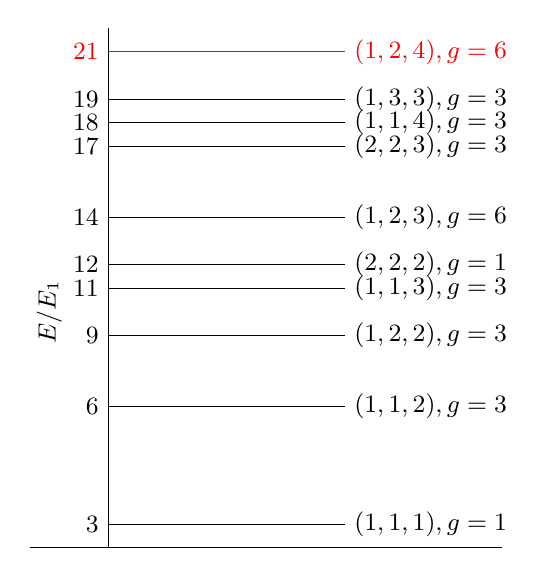
\begin{tikzpicture}
    \draw[-] (-1,0) -- (5,0);
    \draw[-] (0,0) -- (0,6.6);
    \draw[-] (0,0.3) node[left]{\small$3$} -- (3,0.3) node[right]{\small$(1,1,1),g=1$};
    \draw[-] (0,1.8) node[left]{\small$6$} -- (3,1.8) node[right]{\small$(1,1,2),g=3$};
    \draw[-] (0,2.7) node[left]{\small$9$} -- (3,2.7) node[right]{\small$(1,2,2),g=3$};
    \draw[-] (0,3.3) node[left]{\small$11$} -- (3,3.3) node[right]{\small$(1,1,3),g=3$};
    \draw[-] (0,3.6) node[left]{\small$12$} -- (3,3.6) node[right]{\small$(2,2,2),g=1$};
    \draw[-] (0,4.2) node[left]{\small$14$} -- (3,4.2) node[right]{\small$(1,2,3),g=6$};
    \draw[-] (0,5.1) node[left]{\small$17$} -- (3,5.1) node[right]{\small$(2,2,3),g=3$};
    \draw[-] (0,5.4) node[left]{\small$18$} -- (3,5.4) node[right]{\small$(1,1,4),g=3$};
    \draw[-] (0,5.7) node[left]{\small$19$} -- (3,5.7) node[right]{\small$(1,3,3),g=3$};
    \draw[-,red] (0,6.3) node[left]{\red{\small$21$}} -- (3,6.3) node[right]{\red{\small$(1,2,4),g=6$}};
    \node[rotate=90] at (-0.75,3) {\small$E/E_1$};
\end{tikzpicture}
\end{document}